%\section{Maximizing Parallelism}

%\section{Customizable Consistency Constructor (\name)}
\section{Customizable Consistency Generator}
\label{sec:overview}

%\wxzc{ 
%Outline:
%
%1. the problem can be reduced to a verification problem. why? Questions: 1) uncertainty->a number of simultanenous possible views; 2) a number of possible sequence updates;
%
%2. to Q1, existing verifiers don't consider uncertainty, effectly assume ...;
%
%3. to Q2, heuristic..., fallback ...;
%
%4. Figure 1
%}

%\wxzc{what: General consistency properties

%how: our system is designed as a wrapper around a verificaiton engine -- the verificaiton engine can take as input arbitrary invariants -- since we treat the VE as a black box, we can use it to implement arbitrary consitency properites}
%
%Ultimate goal: handle generilized consistency properties efficintly
%
%Approach: uncertainty-aware modelling, black-box verification, synthesis algorithm
%
%In this section, we provide an overview of our system, \name.
%
%Workflow:
%
%Step1: verification
%
%Step2: enforce correctness, algorithm
%
%\label{sec:structure}

\name works by converting the update scheduling problem into a network verification problem, in which arrows indicate flows of network messages (updates or acknowledges).  
%To efficiently enforce consistency of network-wide invariants and policies as
%network states evolve, we convert the complex update scheduling problem into a
%well-defined network verification problem. 
Our overall approach is shown in Figure~\ref{fig:structure}.
Our uncertainty-aware network model (\S\ref{sec:model}) provides a compact symbolic
representation of the different possible states the network could be in,
providing input for the verification engine.
%models the inputs for the verification engine
%Figure~\ref{fig:structure} depicts the system architecture
%Our
%uncertainty-aware network model produces inputs for the verification engine, in
%a manner that accurately captures the network uncertainty (\S\ref{sec:design}). 
The verification engine is responsible for verifying 
application updates against {\em any} specified
invariants and policies (\S\ref{sec:verify}). 
Based on verification results, \name synthesizes an
efficient update plan to preserve policy consistency during network updates,
using the basic heuristic and a more heavyweight fallback mechanism as backup 
(\S\ref{sec:parallelism} and \S\ref{sec:synthesis}).  
One key feature of \name is that it operates in a {\em black-box} fashion, providing
a general platform with a very flexible notion of consistency.
For example, one can 
%One key feature of \name is that as a platform, it
%operates in a black-box fashion, offering a very flexible notion of
%consistency. Therefore, one can 
``plug in" a different verification
function and an update scheduling tool to meet one's customized needs.
%A key feature of \name is that it runs both the verification engine and
%the fallback mechanism in a black-box fashion.  That is, one can plug in
%different checking functions and update tools to leverage the flexible support
%for invariant checking that our general network model provides, and the
%consistency properties those update tools guarantee, respectively.

\begin{figure}[!ht]
  \centering
  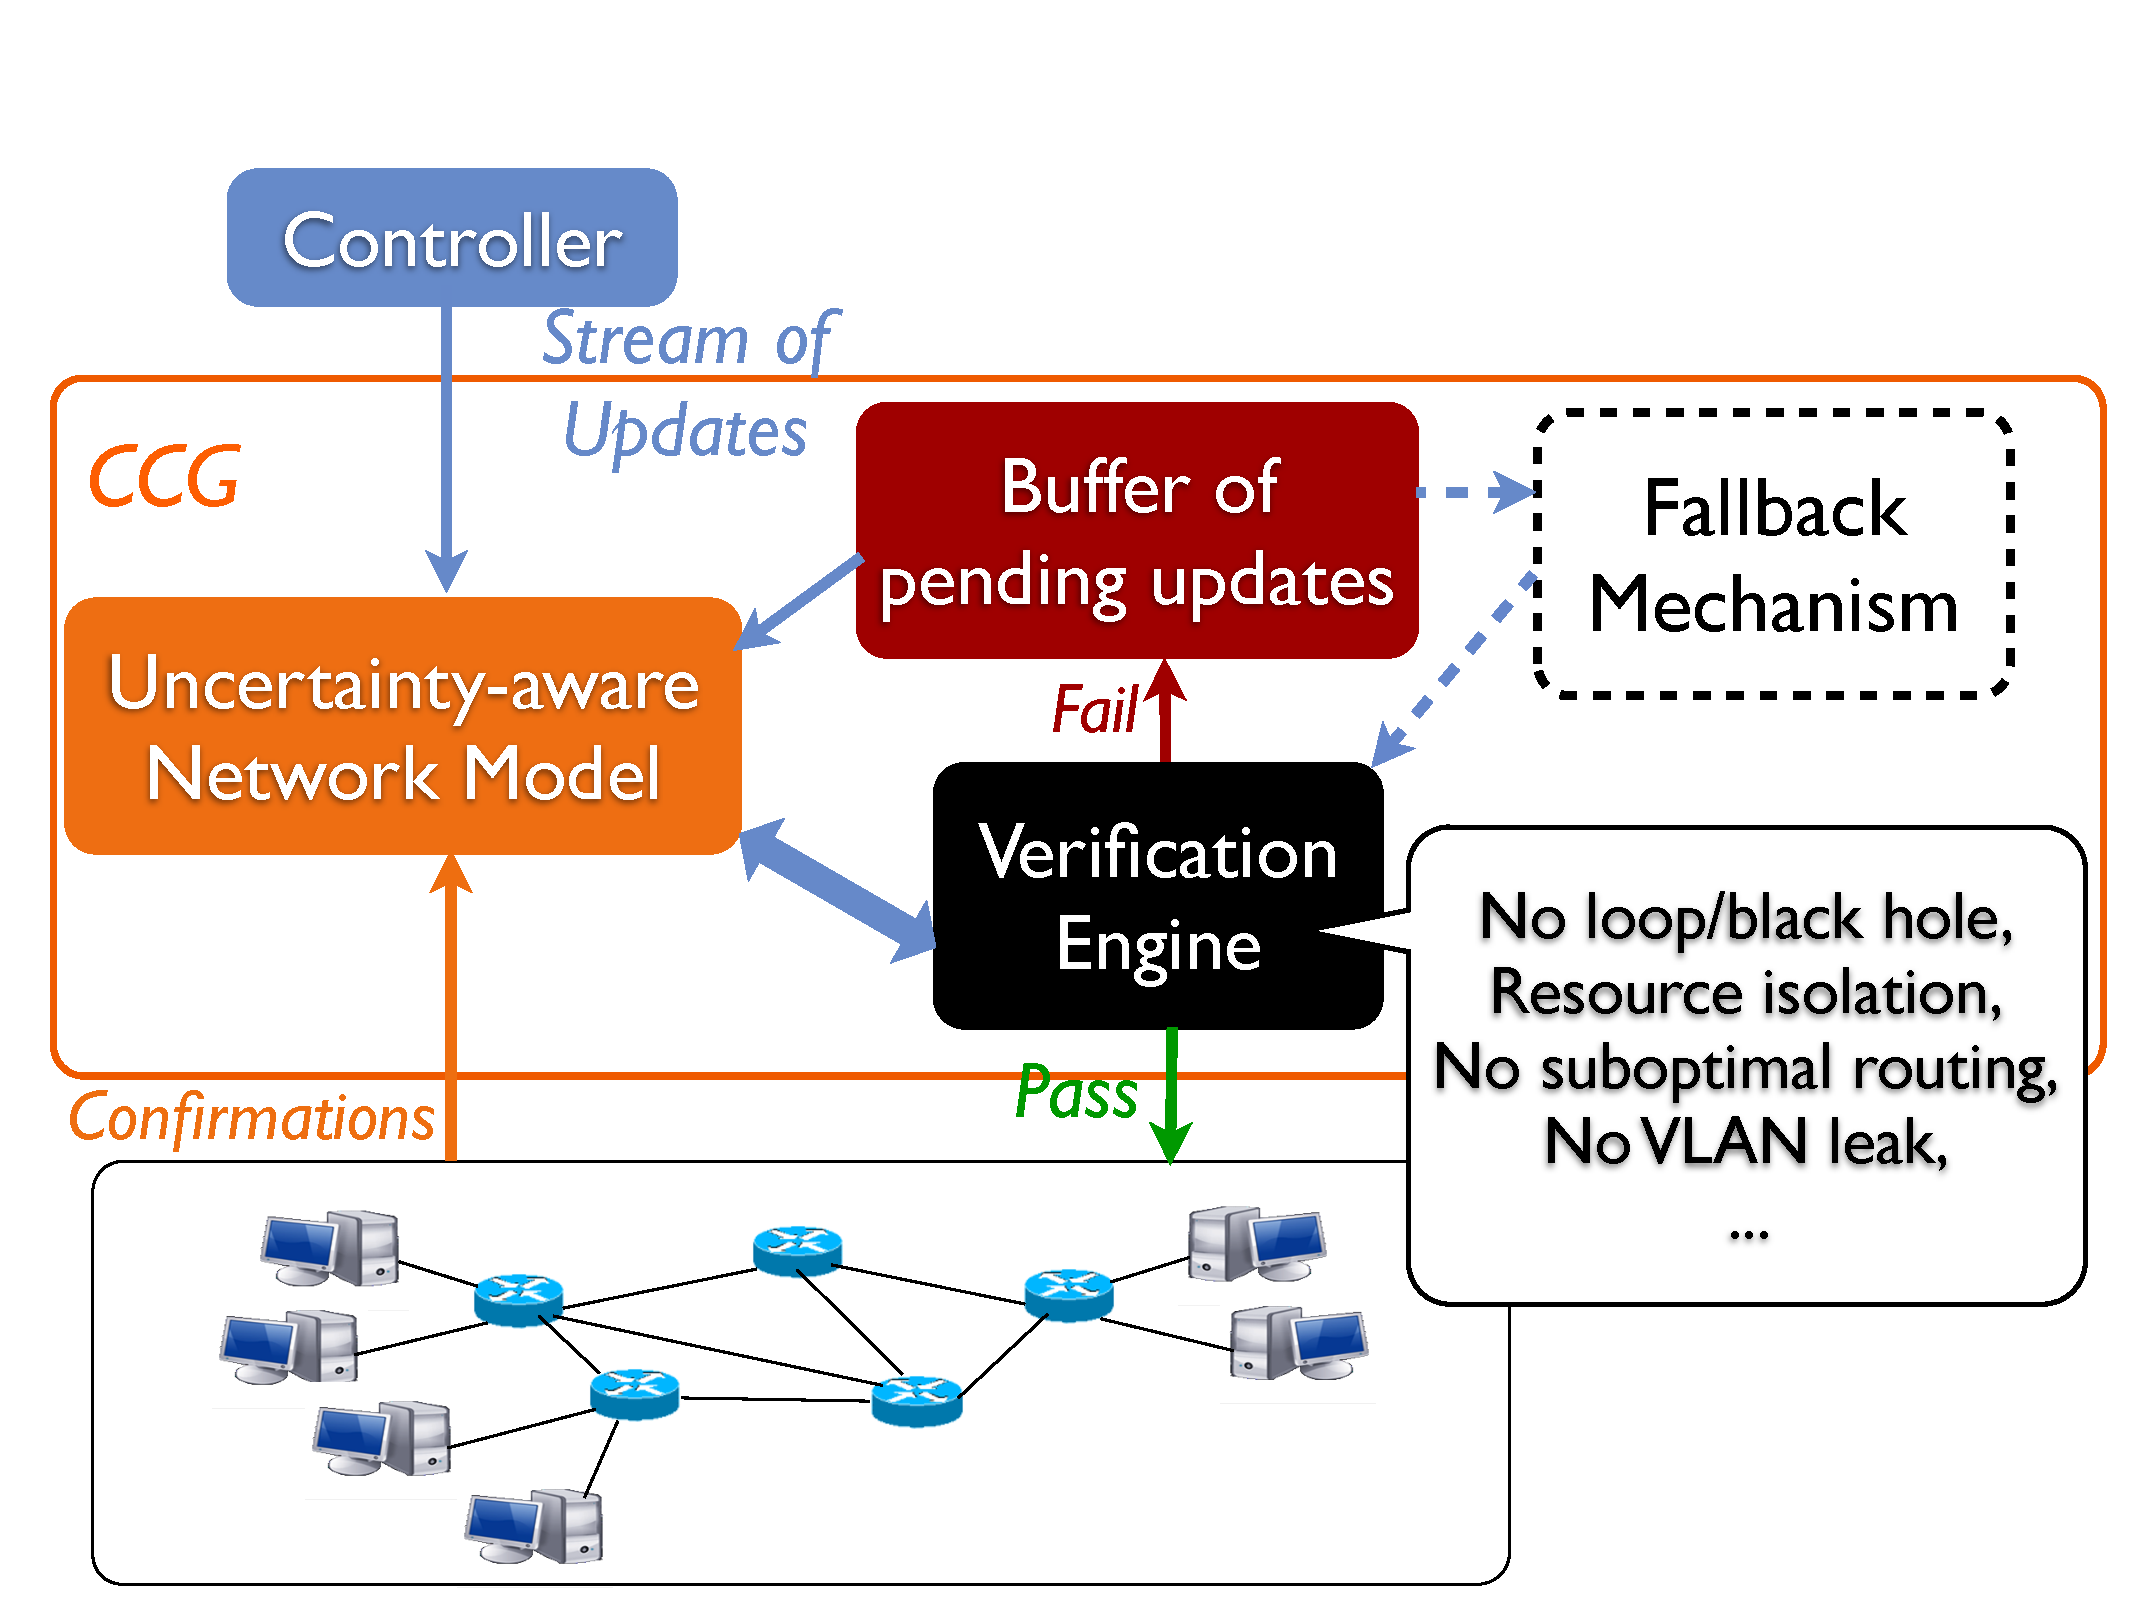
\includegraphics[scale=0.2,trim=0 0 0 1cm]{figs/structure_new}
  \vspace{-0.1in}
  \caption{\em \small System architecture of \name.}
  \vspace{-0.2in}
  \label{fig:structure}
\end{figure}

%  \if 0
%As discussed in \S~\ref{sec:motivation}, guaranteeing generalized consistency properties with maximized efficiency is important, yet difficult.  
%  \cut{
%  Achieving stronger consistency properties may require slowing of the process of updating
%  the data plane, thus harming convergence time and reaction speed.  To achieve a good
%  tradeoff between consistency and efficiency, recent work~\cite{Mahajan13}
%  proposed a scheme to maximize update speed in the context of preserving loop
%  freedom. However, that approach, while useful, provides an algorithm tailored to achieve just a single goal, loop freedom, instead of supporting general
%  consistency properties.  In contrast, our work aims to provide a flexible framework.}
%allowing custom specification of consistency properties, and an algorithmic approach
%to enforce them with good efficiency.


 %and is hence not capable of supporting general consistency properties. In contrast, our work aims to develop a {\em general} framework, which 
%supports a more arbitrary set of consistency properties to be 
%
%The stricter the desired consistency property is,
%%(e.g., packet coherence is a stricter requirement than loop freedom), 
%the slower the data plane can be updated to preserve it.
%To achieve a better consistency-efficiency tradeoff, specific mechanisms that guarantee specific properties
%are proposed. For example, an algorithm tailored for the property of loop freedom is designed to achieve minimal dependency among rules, and thus maximized update speed under the property~\cite{Mahajan13}.
%Such specified tool is useful, but not capable of supporting general consistency properties.
%Thus, a general framework that supports customized property is desired. 
  \if 0
%\wxznew{
%  The problem of enforcing generalized consistency with\cut{ maximized} \wxznew{high} efficiency, 
%  we show, can be reduced to a general verification problem.
%  In particular, the problem of determining a schedule of 
%  when to send updates can be reduced to checking, 
%  with a network verification tool, whether the
%  schedule produces a network that obeys a provided set of consistency invariants.
%  
%  However, checking every possible update ordering would be really
%  inefficient. What's more, even at a single time point, due to the inherent ``network uncertainty" (defined later in \S\ref{sec:design}),
%  one has to check all possible views of the network at that moment to rule out any possiblity of violating policies.
%  \fi

\kevin{
To efficiently enforce general consistency properties on network-wide state,
we convert the update scheduling problem into a network verification problem.
One way to do this would be to enumerate all possible update orderings, and run a
network verification tool~\cite{VeriFlow, NetPlumber2013} after each update, for each possible ordering.
If the network verifier fails on an update, we reject the sequence.

However, this approach would not be very efficient, as the number of possible update orderings
can be large, growing exponentially with the number of queued updates.
 %verifying every possible update ordering would be very inefficient. 
Moreover, this space may be even larger---even at a single instant in time, 
the inherent ``uncertainty" the controller has in the
current state of the network complicates things further. For example,
if the controller recently sent an update, but has not yet received an
acknowledgment, the controller may not be sure what state the network
is currently in. Based on the knowledge it does have the controller
may be able to enumerate the set of possible states the network may be
in, but it must check all of these possible states to rule out the
possibility of violating the consistency policies. This number of states can again
be large (increasing exponentially with the number of unknown forwarding table entries,
for example), and hence such an approach would not be efficient.
%Moreover, at any instance of time, due to the inherent ``network uncertainty" (defined in \S\ref{sec:design}), one has to check all possible views of the network to eliminate any possible policy violations.
}
%Because
%of the distributed nature of networks, the \name engine is unaware of the precise ordering and timing with which updates arrive at devices in the network. To address that, \name explicitly models the “uncertainty” about network state through the use of a novel symbolic network repre- sentation, a data structure that compactly represents all different possible network states.

%in the sense that a
%general network verifier would be able to determine whether any update is safe to pass
%to the network at any time.  
%Using that information, we could greedily
%proceed with network state transition, and heuristically achieve maximized update
%parallelism.

On top of all this, we
%Because of these challenges, we
cannot utilize existing network verifiers, such as VeriFlow~\cite{VeriFlow} and~\cite{PHA2012}
, which inaccurately assume 
%To deal with the \cut{multiple }simultaneous possible network views, \cut{unfortunately, }we cannot utilize 
%existing network verifiers, such as VeriFlow~\cite{VeriFlow} or HSA~\cite{PHA2012}, 
%which effectively yet inaccurately assume 
that updates are applied
at the exact moment when the verification tools see them.
Tools such as VeriFlow and HSA only check
static network snapshots, and do not consider temporal uncertainty
during the transition between snapshots, which can lead to false
positives and false negatives in their diagnoses in practical
settings.
%In other words, they only check static network snapshots, and do not consider
%causing these network models to be inaccurate to some extent.
%temporal uncertainty during the transition of the snapshots.

To deal with these challenges,
\name explicitly models the {\em uncertainty} about network state 
with a novel symbolic network representation --- a data structure that compactly represents all different possible network states. 
%\wxzc{same text as in intro now, need to be changed later.}
%compactly storing the diffiernet options using your symbolic network
%representation and traversing it. 

However, another challenge remains. How can we efficiently find a feasible update sequence that preserves
the desired policies among all possible sequences?
%\cut{while updating the network efficiently. For efficiency purpose, }
To address this, \name uses a greedy heuristic algorithm.
The algorithm utilizes the network verifier to determine whether an update is safe to pass to the network at a given time, if it is it passes it to the network, if not it buffers it.
Upon receiving new information (new updates, acknowledgments from network), it re-checks and attempts to re-send buffered updates.
Our heuristic attempts to maximize parallelism, by automatically determining which update groups could ``conflict'' in the network (in the presence of uncertainty). 
%\kevin{The algorithm utilizes the network verifier to determine whether an update is safe to pass to the network at a given time; it then greedily processes the network state transition, and heuristically maximizes the parallelism of updating the network. 
We formally identify the large scope of consistency policies that are guaranteed by \name's heuristic (\S\ref{sec:seg-independence}). \name achieves high update efficiency (in both speed and memory consumption) by attempting to handle updates with the heuristic, and falling back to other heavyweight techniques (e.g., CU~\cite{Reitblatt2012} and SWAN~\cite{Hong13}) only when necessary (very rare in practice as shown in \S\ref{sec:eval}) to guarantee the provided
set of consistency policies. 

%Figure~\ref{fig:structure} depicts the system architecture. One key feature of \name is that as a platform, it operates in a black-box fashion, offering a very flexible notion of consistency. 
%Therefore, operators can ``plugin" a different verification engine and an update scheduling tool to meet different needs.
}

% \if 0
% as a general network verifier would be able to determine whether any update is safe to pass
% to the network at any time. Using that information, the algorithm 
% greedily proceeds with network state transition, 
% and achieves heuristically maximized update parallelism.
% We formally identify the scope of consistency policies 
% (actually covering a fairly large set of policies) that are guaranteed by 
% \name's heuristic (\S\ref{sec:seg-independence}), and experimentally 
% show its ability to achieve high update efficiency (\S\ref{sec:seg-independence}).
% \name also employs relatively more heavyweight update tools,
% such as CU~\cite{Reitblatt2012} and SWAN~\cite{Hong13},
% as plug-ins. Those plug-ins are triggered only when the heuristic can not find a feasible sequence 
% (very rare as showed in \S\ref{sec:eval}), to ensure supplied consistency policies.
% 
% 
% Figure~\ref{fig:structure} depicts the system architecture. 
% Our uncertainty-aware network model produces inputs for the verification engine, in a
% manner that accurately captures the network uncertainty.
% The verification is responsible for verifying application updates against {\em any} specified invariants and policies.  
% Based on verification results, \name synthesizes an efficient update plan to 
% preserve policy consistency during network updates,
% using the basic heuristic and a more heavyweight fallback mechanism as back up. 
% A key feature of \name is that it runs both the verification engine 
% and the fallback mechanism in a black-box fashion. 
% That is, one can plug in different checking functions and update tools to
% %Doing so enables \name to 
% leverage the flexible support for invariant checking that our general network
% model provides, and the consistency properties those update tools guarantee, respectively.
% \fi
%}

% \if 0
% However, two key challenges remain. First, existing network verification tools, such as 
% %In order to enforce general consistency properties, \name is designed as a wrapper around a \matt{{\em verification engine}, such as 
% VeriFlow~\cite{VeriFlow} and HSA~\cite{PHA2012}, only check static network snapshots against desired properties, and do not consider
% the dynamics inherent in the network.  
% Second, a greedy algorithm such as the one we describe above could get stuck,
% % \mattc{todo:how?}, 
% and then either the whole system would be paused, or
% the \cut{specified} desired consistency properties would be violated.
% 
% %\wxz{Note that there are scenarios where no combination of updates ordering can support the required policy~\cite{Reitblatt2012}. That is, some buffered updates could never be safe to pass to the network.
% To address the first challenge, we designed a network modeling technique that is aware of dynamic settings of the network (\S\ref{sec:design}).
% %Specifically, taking into account the controller's inherent uncertainty about the current state of the network, 
% %\name maintains an {\em uncertainty-aware network model}. 
% That network model \cut{is used to }produces inputs for the verification engine, in a
% manner that accurately captures \wxznew{the dynamics}.%this uncertainty.
% \fi
\if 0
\wxznew{
Due to the second challenge, we adopt a hybrid approach for the design, depending
on the consistency requirement.
As we will show in \S\ref{sec:seg-independence} and \S\ref{sec:eval}, there are
a group of consistency policies, which covers a fairly large set of common policies,
can be guaranteed by the greedy heuristic of \name. 
Hence in this case, we expose the verification engine to application directly, 
ensuring the desired policies while introducing zero extra overhead.
As for policies fall out of this group, thanks to existing update mechanisms,
some of them can be guaranteed if the operators are willing to suffer additional storage
or time overhead. 
Under such circumstances, a layer between the controller applications 
and \name, translation layer, is triggered. 
%In that case, we can adopt two possible alternatives. 
%One is to insert a layer of existing update mechanism, like that proposed in Reitblatt et al.~\cite{Reitblatt2012}, which guarantees the required policy.% between control applications and \name. 
The stream of updates from the application is first fed into 
the translation layer to be transformed to a feasible update sequence. 
Then \name greedily sends updates as long as the policy is preserved. 
In this way, \name is guaranteed to preserve
%correctness is maintained all the time at the cost of extra control overhead and device memory. In other words, \name is able to maintain 
the same level of consistency as the mechanism used in the inserted layer.
This approach suffers an added cost of adding an amount of control and device
memory overhead equivalent to that if using that mechanism separately, but
retains the advantage of greatly shortened the update delay.  Because of the
shorter delay, the period of time that network suffers from heavy memory
overhead is reduced.  
Alternatively, if the operators value update efficiency, and only ask for best-effort to 
maintain consistency during updates, the translation layer won't be triggered, 
but instead, after a configurable threshold, buffered commands are released to the network (\S\ref{sec:parallelism}).
That is, operators have a choice of balancing efficiency and consistency trade-off.
%However, maintaining properties does not necessarily
%require use of such a layer, as we later show in \S\ref{sec:eval}.
}
%However, there are properties, assurance of which don't require such a heavy layer, as we show~\ref{sec:eval}.
%Hence another alternative is to expose the verification engine to application directly, which reduces control and device memory overhead further.
%, sacrifice correctness to some extent but maintains high efficiency. For example, to limit disruption on network operations, the network operator can specify a timeout value, upon on the expiration of which a buffered update is issued.}
\wxzc{Change to one approach. Fall-back mechanism: issue the buffered updates
after a threshold of waiting time use 2-phase update.}

\kevin{
To address the second challenge, we began by formally identifying the scope of consistency policies 
(actually covering a fairly large set of policies) that are guaranteed by 
\name's heuristic (\S\ref{sec:seg-independence}).
%never get stuck with \name's greedy heuristic. 
\cut{The performance is extremely fast because of the direct interaction between the verification engine and the applications. }
For policies outside that scope, our approach is to integrate \name's
heuristic with existing update mechanisms in the following way. Upon
receiving network updates from applications, \name greedily sends updates as
long as the desired policy is preserved. Whenever \name gets stuck on an
update, it automatically falls back to other consistent update tools, such as
CU~\cite{Reitblatt2012} and SWAN~\cite{Hong13}. 
Thus, our algorithm guarantees the same level of
consistency as the existing solutions do. 
\cut{The hybrid approach is slower than \name, but not surprisingly so; it still greatly shortens the update delay and
reduces the memory overhead, compared to CU~\cite{Reitblatt2012} and SWAN~\cite{Hong13} used alone.} 
%Alternatively, if the operators value update efficiency, and only ask for best-effort to 
In fact, in many cases, network operators value updates efficiency (e.g., speed), 
and only ask for the best-effort to maintain consistency.
%without losing too much efficiency during network updates. 
Then \name is able to offer the flexibility to balance between efficiency and consistency
through a configurable timing threshold, over which buffered commands are simply
released to the network.}
\fi

\if 0
\name consists of the following components, as shown in
Figure~\ref{fig:structure}: an uncertainty-aware network
model\cut{(\S\ref{sec:design})}, a translation layer, a black-box verification
engine, and a data structure that buffers problematic updates temporarily. 
%The translation layer produ \mattc{missing text?}
The verification engine leverages the network model, and is responsible to
verify updates against {\em any} specified invariants.  Based on verification
results, \name provides an algorithm to synthesize a correct and efficient update plan,
\wxznew{with the help of the translation layer when necessary}.
\fi

%for when, where, and how to release buffered updates to the network
%(\S\ref{sec:parallelism}).

%Doing so enables \name to make direct use of these tools' capabilities of checking (but not instilling) correctness properties.}

%Second, it is difficulty to support an \emph{arbitrary}\wxzc{should we say "arbitrary" or be a little conservative here?} consistency property.
%If the policy verification function is tightly coupled with other components, 
%whenever a different policy is desired, we end up redesign the entire system. 
%To this end, we design a platform, which takes the decision procedure of 
%any property of interest as a plug-in module 
%rather than reasoning a specific property invariant.
%We name this plug-in module as black-box verification engine.
%Given an update and a network model as inputs, 
%a black-box engine simply outputs whether or not this update passes the specific verification.
%%For any given consistency requirement, for example, two hosts c , or no suboptimal routes, 
%%is specified as a verification engine plugged into the framework. 
%Based on the outputs, we design an algorithm to synthesize an update plan 
%compliant with the property while maximizing update parallelism.
%In this way, we are able to realize flexible network consistency notion.
%%without any knowledge of internal workings of the verification engine.
%\paragraph{Uncertainty-aware network model}

%\paragraph{Black-box verification engine}
%\if 0
%A key property of \name is to run the verification engine in a black-box fashion.
%Doing this enables \name to leverage the flexible support for invariant checking
%that existing network verifiers already provide.
%\name assumes the verification engine operates in a per-update fashion (a la Veriflow, NetPlumber, and FlowChecker~\ref{Al-Shaer2010}). \wxz{For each update, it takes the update as well as a graph representing network states, such as our network model(\S~\ref{sec:design}) as inputs}, and outputs a {\em pass} if the update does not violate invariants, and a {\em fail} otherwise.
%\mattc{Wait a second... you don't really use the verifier as a black box right? You need to feed that symbolic graph into it. Don't you need to extend the verifier to deal with symbolic links? If so you need to describe that briefly here, and maybe tone down "black box".}
%\name then uses this output to synthesize an update ordering that obeys the provided set of correctness
%invariants.
%To do this, \name retains a buffer of updates -- if an update fails the verification process,
%it can be buffered until a point where the update becomes safe to send. \mattc{what if this never happens? do you eventually discard? where do you discuss this in the paper?}
%\mattc{I didn't understand a lot of the paragraph that was here so I cut it -- is what I wrote above missing anything you wanted to say? your paragraph is commented out here:}
%\if
% Inspired by black-box testing techniques, the verification functionality in \name is designed as a black-box \matt{unit within} our network model\mattc{I don't see how it's inspired by that in particular}.
% \name takes the decision procedure of any properties of interest as a plug-in module rather than reasoning a specific property invariant\mattc{I can't parse this sentence, what does it mean?}.
% We name that plug-in module as black-box verification engine.
% %If the policy verification function is tightly coupled with other components, 
% %whenever a different policy is desired, we end up redesign the entire system. 
% The design goal is to support arbitrary invariants. Once a invariant or a set of invariants is specified, a corresponding verification engine is plugged into \name. The verification engine takes the network model and network updates as inputs, and examines whether applying the updates to the model could violate the invariants. 
% That is, we do not need to peer into its internal structures and workings, 
% or modify any other modules of \name.
% In addition, programmers can write their own checkers with the unified interfaces.
% For each update, the verification engine simply outputs whether or not the update violate any invariant.

%The outputs of the verification engine are 
%(1) whether or not the update violates the invariant(s), and 
%(2) all the possible locations where that update fails the verification, i.e., the possibility of safely issuing that update later relies on the status of some future or in-flight updates on those locations.
%Note that it is the invariant that determines the dependencies among updates.
%Note that such dependencies vary as invariants change.
%Take Figure~\ref{fig:dependency} as an example...
%
%loop
%
%black hole

%\paragraph{Dependency graph buffer}
%We develop a graph type data structure to temporarily store updates that don't pass the verification. The reason that a graph is used here, is to present the dependency between updates. As stated above, invariants determine the dependency relationships among updates, 
%and the verification engine outputs such relationships to the dependency graph.
%From any location that a buffered update is relying on to this update there is a directed link. Any future change on one of the locations will activate reprocessing of this update, 
%to see if it's the time to pass it to the network. More details are in \S~\ref{sec:algo}. 
\fi

